%%%%%%%%%%%%%%%%%%%%%%%%%%%%%%%%%%%%%%%%%
% Simple Sectioned Essay Template
% LaTeX Template
%
% This template has been downloaded from:
% http://www.latextemplates.com
%
% Note:
% The %\lipsum[#] commands throughout this template generate dummy text
% to fill the template out. These commands should all be removed when 
% writing essay content.
%
%%%%%%%%%%%%%%%%%%%%%%%%%%%%%%%%%%%%%%%%%

%----------------------------------------------------------------------------------------
%	PACKAGES AND OTHER DOCUMENT CONFIGURATIONS
%----------------------------------------------------------------------------------------

\documentclass[10pt]{article} % Default font size is 12pt, it can be changed here

\usepackage[spanish]{babel}%Para el español
\usepackage[utf8]{inputenc}%para los acentos
\usepackage{amsmath,amssymb,amsfonts,amsthm}
\usepackage{graphicx}
\usepackage{bbm}
\usepackage{textcomp}
\usepackage{amstext}

\usepackage{geometry} % Required to change the page size to A4
\geometry{a4paper} % Set the page size to be A4 as opposed to the default US Letter

\usepackage{graphicx} % Required for including pictures

\usepackage{float} % Allows putting an [H] in \begin{figure} to specify the exact location of the figure
\usepackage{wrapfig} % Allows in-line images such as the example fish picture

\linespread{1.2} % Line spacing

%\setlength\parindent{0pt} % Uncomment to remove all indentation from paragraphs

\graphicspath{{Imagenes/}} % Specifies the directory where pictures are stored

%\usepackage{tikz}
%%%<
%\usepackage[spanish]{babel}%Para el español
%\usepackage[utf8]{inputenc}
%\usepackage{verbatim}
\usepackage{listings}
%\usepackage{xcolor}


%\usepackage{times}
 
%\definecolor{dkgreen}{rgb}{0,0.6,0}

\lstset{
	language=C,
	literate=%
	{á}{{\'{a}}}1
	{é}{{\'{e}}}1
	{í}{{\'{i}}}1
	{ó}{{\'{o}}}1
	{ú}{{\'{u}}}1
	{ñ}{{\~{n}}}1
	{<}{{$<$}}1
	{>}{{$>$}}1,
	basicstyle=\footnotesize\ttfamily,
	keywordstyle=\bfseries, 
	comment=[l]{\;},%
	breaklines=true,
	prebreak = \raisebox{0ex}[0ex][0ex]{\ensuremath{\hookleftarrow}},
    }

\usepackage{framed}
\usepackage{tabularx,colortbl}
\usepackage{adjustbox}
\usepackage{pdflscape}

\begin{document}


%----------------------------------------------------------------------------------------
%	TITLE PAGE
%----------------------------------------------------------------------------------------

\begin{titlepage}
\newgeometry{left=1.5cm,right=1.5cm}

\newcommand{\HRule}{\rule{\linewidth}{0.5mm}} % Defines a new command for the horizontal lines, change thickness here

\center % Center everything on the page

\textsc{\LARGE Universidad Nacional de Córdoba}\\[1.5cm] % Name of your university/college
\textsc{\Large Informe Trabajo Final}\\[0.5cm] % Major heading such as course name
\textsc{\large Ingeniería de Software}\\[0.5cm] % Minor heading such as course title

\HRule \\[0.4cm]
\Large{ \huge \bfseries Aplicación de las técnicas de Ingeniería de Software sobre un proyecto inconcluso.}\par % Title of your document
\HRule \\[1.5cm]

\begin{minipage}{0.5\textwidth}
\begin{flushleft} \large
\emph{Autores:}\\
Crístian \textsc{Gutierrez} (35.104.714)\\
Esteban \textsc{Morales} (35.104.714)\\
Fabiola \textsc{Campos} (35.258.183)\\
Gianfranco \textsc{Barbiani} (33.414.224)\\
\end{flushleft}
\end{minipage}
~
\begin{minipage}{0.4\textwidth}
\begin{flushright} \large
\emph{Supervisor:} \\
Ing. Martín \textsc{Miceli}
\end{flushright}
\end{minipage}\\[4cm]

{\large \today}\\[3cm] % Date, change the \today to a set date if you want to be precise

%\includegraphics{Logo}\\[1cm] % Include a department/university logo - this will require the graphicx package

\vfill % Fill the rest of the page with whitespace
\restoregeometry
\end{titlepage}

%----------------------------------------------------------------------------------------
%	TABLE OF CONTENTS
%----------------------------------------------------------------------------------------

\tableofcontents % Include a table of contents

\newpage % Begins the essay on a new page instead of on the same page as the table of contents 

%----------------------------------------------------------------------------------------
%	INTRODUCTION
%----------------------------------------------------------------------------------------

\begin{abstract}
En el presente informe se expone el desarrollo del trabajo final para la cátedra Programación Concurrente que se cursa en el primer cuatrimestre del cuarto año de la carrera Ingeniería en Computación en la Facultad de Ciencias Exáctas Físicas y Naturales de la Universidad Nacional de Córdoba, Argentina. 
Este trabajo tiene por consigna la simulación de una celda flexible de producción mediante el modelado por redes de petri y la implementación concurrente programada en Java. Tal implementación incluye la programación de los procesos productivos que ejecutan sus tareas de forma paralela y el diseño de un monitor para garantizar la sincronización de la adquisición y devolución de los recursos compartidos.

\end{abstract} % Major section

\section{Nota de Entrega}

\subsection{Listado de Funcionalidad}

\subsection{Pass/Fail Ratio del Sistema (PFR)}

\subsection{Bugs Conocidos}

\subsection{Vínculo a las fuentes del proyecto}

\section{Manejo de Configuraciones}

\subsection{Plan de Manejo de las Configuraciones}

\subsection{Herramienta de Control de Versiones}
Dirección y forma de accesos a la herramienta de control de versiones

\subsection{Sobre los Directorios}
Esquema de Directorios y propósito de cada uno.

\subsection{Etiquetado y Nombramiento de Archivos}
Normas de etiquetado y de nombramiento de los archivos

\subsection{Plan del Esquema de Ramas}

\subsection{Políticas de Marge y de Etiquetado de Progreso.}
Políticas de fusión de archivos (o sea mergeo) y de etiquetado de acuerdo al progreso de calidad en los entregables.

\subsection{Sobre los Releases}
Forma de entrega de los “releases”, instrucciones mínimas de instalación y formato de entrega.

\subsubsection{Forma de Entrega}

\subsubsection{Instrucciones de Instalación}

\subsubsection{Formato de Entrega}

\subsection{Integrantes}
Listado y forma de contacto de los integrantes del equipo, así como sus roles en la CCB. También incluir periodicidad de las reuniones y miembros obligatorios.
\subsubsection{Roles}
\subsubsection{Sobre las Reuniones}

\subsection{Herramienta de Seguimiento de Errores}
Herramienta de seguimiento de bugs usado para reportar los defectos descubiertos y su estado.

\subsection{Cualquier otra información relevante}


\section{Requerimientos}

\subsection{Diagramas de Casos de Uso}

\subsection{Diagramas de Secuencias}

\subsection{Requerimeintos Funcionales del Sistema}

\subsection{Requerimeintos No Funcionales del Sistema}

\subsection{Diagrama de Arquitectura Preliminar}

\subsection{Matriz de Trazabilidad}


\section{Arquitectura}

\subsection{Gráfico de Arquitectura}

\subsection{Componentes vs Interfaces Externas}

\subsection{Patrón de Arquitectura}

\subsection{UML de Despliegue}

\subsection{UML de Componenetes}

\subsection{Diagrama de Contexto}


\section{Diseño e Implementación}

\subsection{Diagrama de Clases}
Con el objetivo de modularizar el código y procurar el encapsulamiento de cada parte, se decidió la implementación de las siguientes clases:
\begin{itemize}
\item Actualizador.java
\item Componente.java
\item FinalConcurrente.java
\item Monitor.java
\item PanelControl.java
\item Proceso.java
\item VentanaPanel.java
\end{itemize}
Se muestra a continuación el diagrama de clases y luego se desarrollará una breve descripción de las clases más importantes y se detallan los métodos más relevantes.
\begin{figure}[H] % Example image
\center{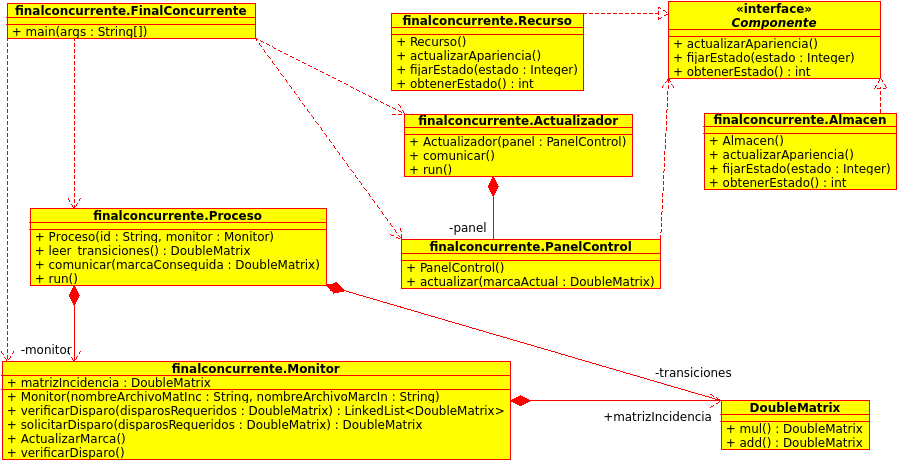
\includegraphics[width=\linewidth]{DiagramaDeClases}}
\label{fig:DiagramaDeClases}
\end{figure}
\subsection{Actualizador}
Es el hilo encargado de actualizar los valores de la pantalla, cada vez que se ejecuta un disparo. Recibe la nueva marca del sistema enviada por el proceso que realizo el disparo, a través de la implementación de Sockets. El actualizador ejecuta el método actualizar de la clase PanelControl con  esta nueva marca.
\subsection{Monitor}
Este objeto es el que se encarga de administrar los recursos del sistema, y determinando los disparos que sean posibles realizar para cada proceso. 
Al inicializarse cargara la configuración del sistema desde un archivo, que contiene la matriz de incidencia. Y desde otro archivo leerá la marca inicial del sistema.
Los métodos principales del monitor son verificarDisparo y solicitarDisparo:
\begin{itemize}
\item SolicitarDisparo():\\Este método es llamado por los procesos, se hace uso de los métodos lock() y unlock() para garantizar la exclusión mutua.
Dentro de este método se llama a verificarDisparo(), que devolverá una lista con todos los disparos que son posibles de efectuarse en ese instante, de entre todos  los permitidos para el proceso.
En caso de no haber disparos posibles, el proceso se duerme en la cola de condición. Si hay disparos posibles, se determina uno al azar, y se dispara actualizando la marca. Luego se despierta a los procesos que estén dormidos en la cola de condición, y por ultimo se libera la exclusión mutua con un unlock().
Se retorna al proceso con una lista de dos elementos, el disparo ejecutado y la nueva marca.
\item VerificarDisparo():\\Este método es llamado desde solicitarDisparo(), recibe un vector que indica las transiciones permitidas para el proceso. Determina cuales son factibles de realizarse, sin que se produzca algún problema de concurrencia (Interbloqueo, inanición). Y retorna una lista con todos los disparos que son posibles de realizarse.
\end{itemize}
\subsection{Proceso}
Se crearan tres hilos que corresponderán a cada linea de producción. Al inicializarce leerán las transiciones que pueden ejecutar desde un archivo. Durante su ejecución solicitaran disparos al monitor, y una vez que el monitor les da los recursos ejecutan el método comunicar(), para que se actualice la interfaz gráfica.

\subsection{Diagrama de Objetos}

\subsection{Diagrama de Sequencia}
A continuación se muestra el diagrama de sequencia de ejecución del proceso.
\begin{figure}[H] % Example image
\center{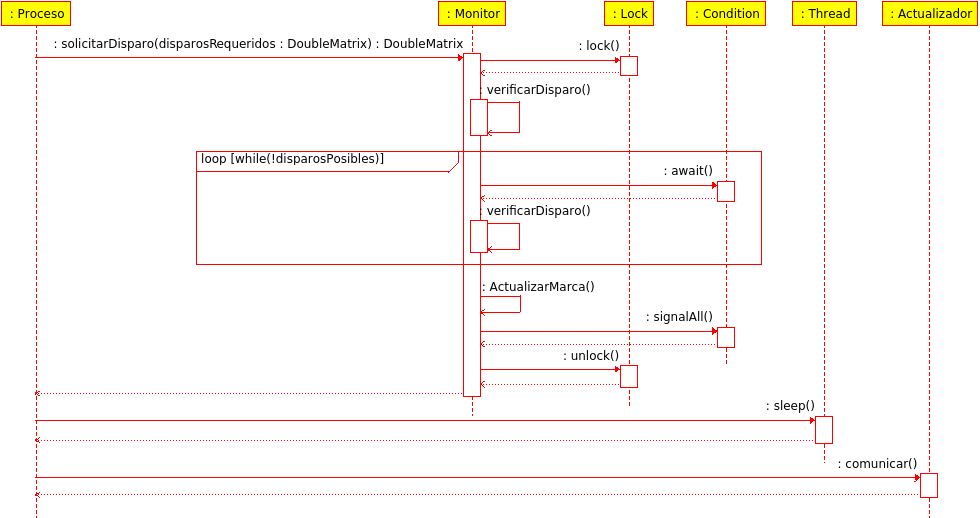
\includegraphics[width=\linewidth]{DiagramaDeSecuencia}}
\label{fig:DiagramaDeSecuencia}
\end{figure}

\subsection{Diagrama de Estados}

\subsection{Diagrama de Paquetes}

\subsection{Patrón de Diseño adicional implementado}

\subsection{Validación del Sistema y Pruebas}
Para validar el sistema se usa el algoritmo iterativo de análisi de Sifones.
Para ello se calculan en el simulador todos los sifones posibles. De todo el conjunto deben discriminarse otros subconjuntos:
\begin{itemize}
\item Conjunto de Sifones que tienen marca inicial distinta de cero.
$$S_{CMI}=\left\{\forall s \in S / t\equiv 0 \wedge s\neq 0\right\}$$
\item Conjunto de Sifones que tienen marca igual a cero al momento del bloqueo.
$$S_{SMB}=\left\{\forall s \in S / t\equiv BLOQ \wedge s\equiv 0\right\}$$
\end{itemize}
La intersección de ambos conjuntos (Sifones que tenían marca al incio de la simulación y están vacíos al momento del bloqueo) son los sifones que deben controlarse o limitarse para poder asegurar la usencia de bloqueos.\\
En el caso de nuestra implementación puede observarse una plaza adicional con marca inicial 3 (tres) que agregamos con este propósito. Así como comentamos en la sección de creación de la red de petri, puede interpretarse como un control necesario para el funcionamiento sin bloqueos.
\begin{figure}[H] % Example image
\center{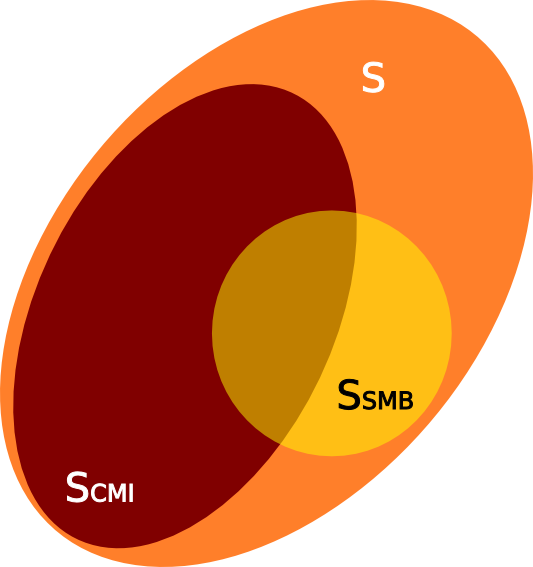
\includegraphics[width=0.4\linewidth]{conjuntos}}
\label{fig:conjuntos}
\end{figure}

\section{Pruebas Unitarias del Sistema}

\subsection{Pruebas Automáticas}

\subsection{Casos de Prueba del Sistema}
\subsubsection{Contra los Requerimientos Funcionales del Sistema}
\subsubsection{Contra los Requerimientos No Funcionales del Sistema}
\subsection{Casos de Prueba Alternativos}

\subsection{Smoke/Sanity Tests}

\subsection{Matriz de Trazabilidad Actualizada}

\subsection{Pass/Fail Ratio por tipo de Caso de Prueba}

\subsection{Bugs Identificados y Corregidos}


\section{Datos Históricos}


\section{Información Adicional}
%------------------------------------------------
\subsection{Descripción del estado inicial del Proyecto (Consigna)}
Sea una planta industrial donde se intenta producir tres tipos de piezas distintas mediante el uso de una celda de producción flexible que incluye tres robots, cuatro máquinas, tres almacenes de materiales y tres almacenes de piezas producidas.
Debe tener en cuenta las siguientes reglas de producción para cada pieza:
\begin{itemize}
\item \textsc{Pieza 1}: Para producir una unidad de pieza (1), una unidad de material del almacen $I_1$ debe someterse a los porcesos de la máquina $M_1$ y la máquina $M_2$. Finalmente se colocan las piezas producidas en el almacen $=O_1$.
$$I_1 \rightarrow M_1 \rightarrow M_2 \rightarrow O_1$$ 
\item \textsc{Pieza 2}: Existen dos reglas para producir una unidad de pieza (2), una unidad de material del almacen $I_2$ debe someterse a los porcesos de la máquina $M_4$ ,la máquina $M_3$ y la máquina $M_1$ ó bien pasar por las máquinas $M_2$, $M_3$ y $M_1$. Finalmente se colocan las piezas producidas en el almacen $=O_2$.
$$I_2 \rightarrow M_4 \rightarrow M_3 \rightarrow M_1 \rightarrow O_2$$
$$I_2 \rightarrow M_2 \rightarrow M_3 \rightarrow M_1 \rightarrow O_2$$
\item \textsc{Pieza 3}:Para producir una unidad de pieza (1), una unidad de material del almacen $I_3$ debe someterse a los porcesos de la máquina $M_3$ y la máquina $M_4$. Finalmente se colocan las piezas producidas en el almacen $=O_3$.
$$I_3 \rightarrow M_3 \rightarrow M_4 \rightarrow O_3$$ 
\end{itemize}
Los encargados de transportar los materiales, productos intermedios y finales son los robots, en este caso se cuenta con tres y cuyas responsabilidades se detallan a continuación:
\begin{itemize}
\item Robot 1 (R1):$[I_1,M_1,M_3,O_2]$
	\begin{itemize}
	\item Carga la máquina $M_1$.
	\item Libera la máquina $M_3$.
	\item Quita materiales del almacen $I_1$.
	\item Deposita las piezas (2) en el almacen $O_2$.
	\end{itemize}
\item Robot 2 (R2):$[I_3,M_1,M_2,M_3,M_4]$
	\begin{itemize}
	\item Libera la máquina $M_1$.
	\item Libera la máquina $M_2$.
	\item Libera la máquina $M_4$.
	\item Carga la máquina $M_3$.
	\item Carga la máquina $M_4$.
	\item Quita materiales del almacen $I_3$.
	\end{itemize}
\item Robot 3 (R3):$[M_2,M_4,0_1,0_3]$
	\begin{itemize}
	\item Carga la máquina $M_2$.
	\item Carga la máquina $M_4$.
	\item Libera la máquina $M_2$.
	\item Libera la máquina $M_4$.
	\item Deposita las piezas (1) en el almacen $O_1$.
	\item Deposita las piezas (3) en el almacen $O_3$.
	\end{itemize}
\end{itemize}
Se pide como consigna modelar el sistema con una red de petri, luego debe programarse la solución y emplearse un monitor para la sincronización de los procesos concurrentes.


%----------------------------------------------------------------------------------------
%	CONCLUSION
%----------------------------------------------------------------------------------------

\subsection{Conclusión} % Major section
El desarrollo del presente trabajo práctico muestra una forma de implementación de una celda de producción flexible a partir del modelo en redes de petri y sincronización de los recursos mediante el uso de un monitor.
Implementar la consigna nos permitió estudiar una alternativa de rápido desarrollo para la construcción de simulaciones.
El uso de un vector de marcas sustituye y encapsula la gestión de los semáforos o condiciones de una forma limpia y sencilla.
El protocolo de disparo de la red se resume al cálculo de marcas posibles por lo que resultó de codificación trivial y segura.\\
\emph{Otra opción válida para evaluar la factibilidad del disparo y el cálculo de la nueva marca es reemplazar la multiplicación de la matriz de incidencia  con el vector de disparo tan solo por el acceso a la colúmna de la matriz respecto del ínidice correspondiente a la transición de disparo.\\
Sin embargo, al implementar la ecuación de forma estrictamente matricial nos permite, en una mejora futura, incluir el procesamiento de prioridades y tiempos específicos en los estados de la simulación.\\}
Los resultados de las simulaciones son consistentes y coherentes. En una somera comparación la simulación de producción de 100 piezas de cada tipo lleva 1802 pasos de simulación mientras que en el simulador que se usó en clases necesita 1800, esto muestra que, en promedio, nuestra implementación alcanza los mismos resultados.
Desde un enfoque industrial este mismo software podría utilizarse como controlador de los tiempos de los procesos y como monitor de permisos para regular el comportamiento de la celda.
%%\lipsum[12-13]

%----------------------------------------------------------------------------------------
%	BIBLIOGRAPHY
%----------------------------------------------------------------------------------------

\begin{thebibliography}{99} % Bibliography - this is intentionally simple in this template

\bibitem[1]{Springer:LNCS6709}
 \textsc{Kristensen, Lars M.} and \textsc{Petrucci, Laure}
\textit{Applications and Theory of Petri Nets}
32nd International Conference PETRI NETS 2011, Newcastle, UK, June 2011

\bibitem[1]{CRC Press:2009dg}
 \textsc{Naiqi Wu} and \textsc{MengChu Zhou}
\textit{System Modeling
and Control with
Resource-Oriented
Petri Nets}
6000 Broken Sound Parkway NW, Suite 300, 2010
\newblock {\em Process- vs. Resource-
Oriented Petri Nets}, 6:71--81.



\end{thebibliography}

%----------------------------------------------------------------------------------------

\end{document}
